\chapter{Architecture Globale et Choix Technologiques}
\label{chap:arch_globale}

\section{Vue d'Ensemble et Décomposition N-Tiers}

La conception architecturale de la plateforme \textbf{Perceptra} obéit à des impératifs d'ingénierie logicielle stricts~: haute modularité, découplage fort entre l'interface utilisateur et le moteur de calcul scientifique, déterminisme des algorithmes de traitement d'images, extensibilité horizontale et simplicité de déploiement.

Pour répondre à ces exigences tout en assurant une expérience utilisateur fluide et sans latence perceptible lors du traitement de requêtes complexes sur 10\,000 images, Perceptra est structuré selon un patron d'architecture distribuée \textbf{N-Tiers} articulé autour d'API RESTful sans état (\textit{stateless}), illustré sur la figure~\ref{fig:system_ntiers}.

\begin{figure}[H]
\centering
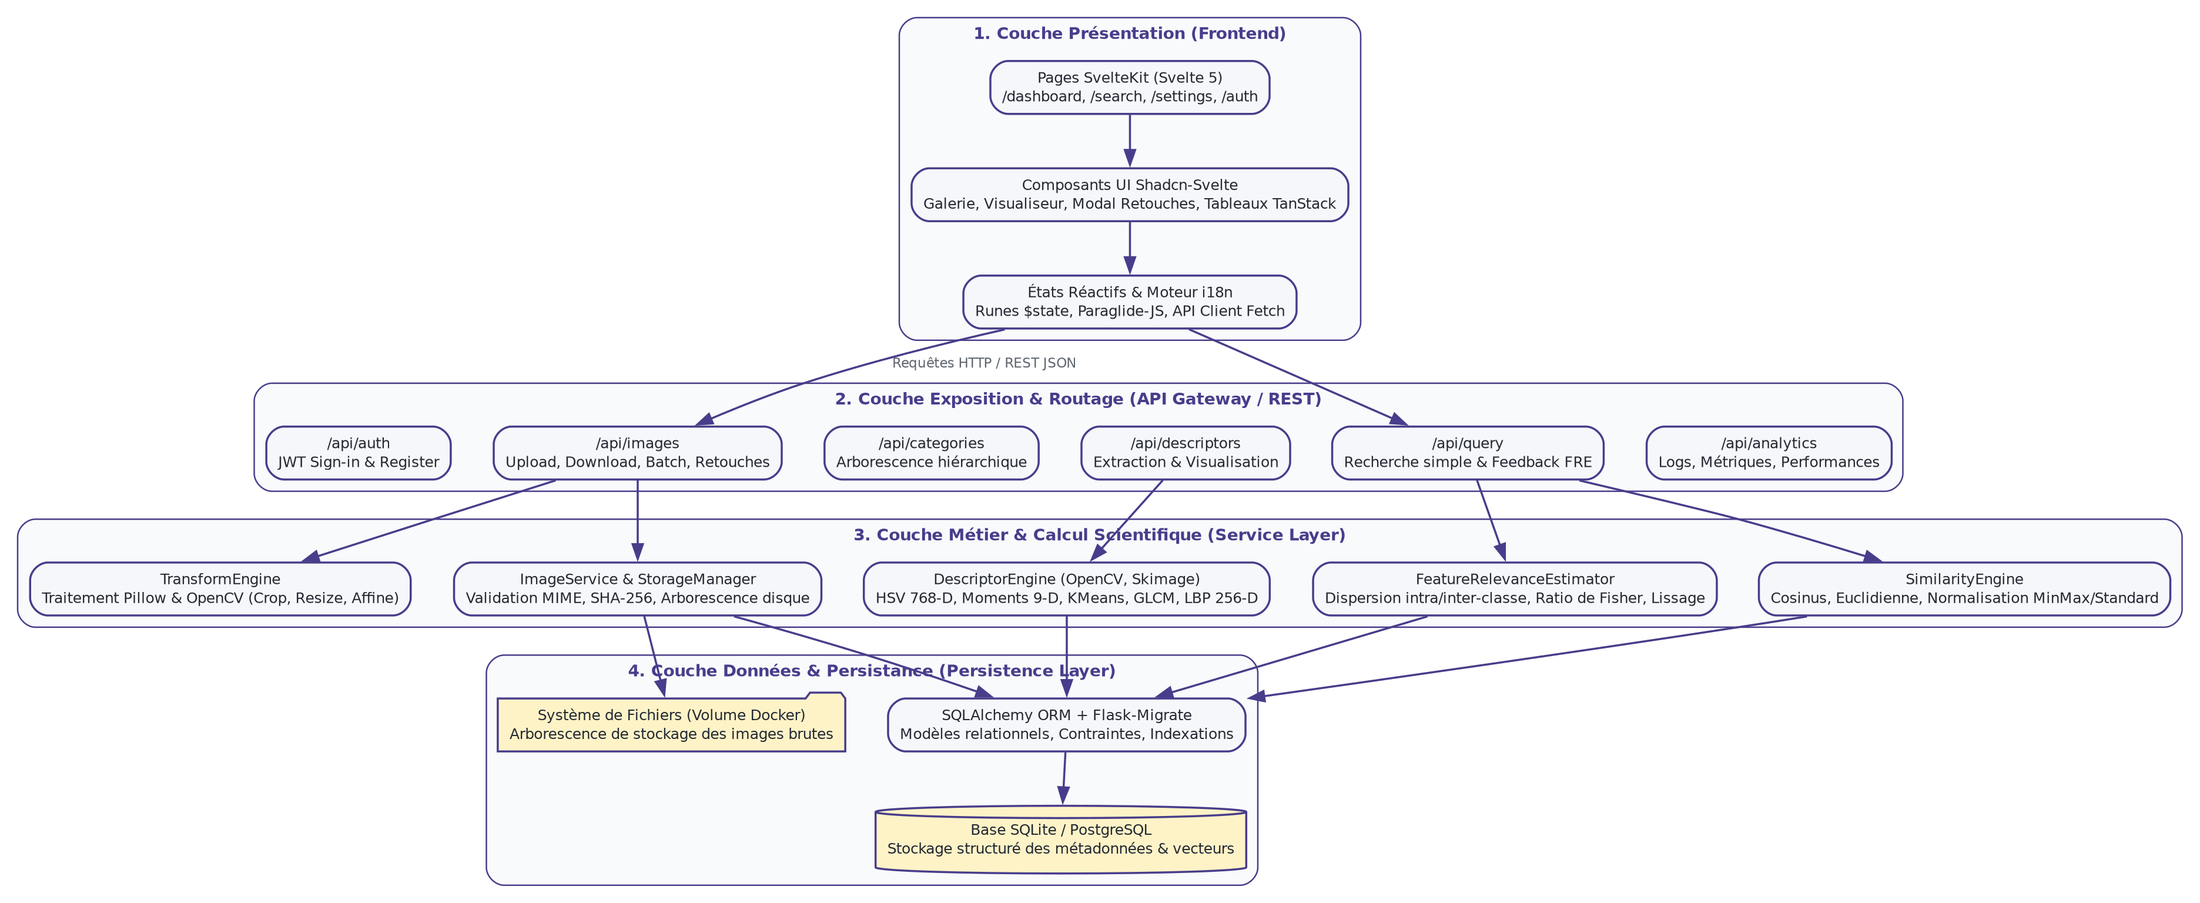
\includegraphics[width=0.78\textwidth]{images/03-architecture-systeme-n-tiers.png}
\caption{Décomposition architecturale globale en couches logiques N-Tiers}
\label{fig:system_ntiers}
\end{figure}

Le système est découpé en quatre strates logiques indépendantes, garantissant une séparation rigoureuse des responsabilités (\textit{Separation of Concerns} -- SoC)~:

\subsection{1. Couche Présentation (Frontend Web)}
Hébergée sur le navigateur du client, cette couche est intégralement construite avec le framework \textbf{SvelteKit 3} exploitant le nouveau moteur de réactivité fine \textbf{Svelte 5} (système des \textit{Runes}~: \texttt{\$state}, \texttt{\$derived}, \texttt{\$effect}). Elle assure l'affichage interactif de la galerie de médias, le studio de retouche d'image non destructif, le tableau de bord de recherche visuelle avec curseurs dynamiques, et l'internationalisation native bilingue (Français/Anglais) propulsée par \textit{Paraglide-JS}.

\subsection{2. Couche Exposition et Routage (Passerelle API REST)}
Cette couche constitue le point d'entrée unique des communications client-serveur. Elle est orchestrée par le serveur WSGI de production \textbf{Gunicorn} relayé par un reverse proxy \textbf{Nginx} ou le serveur de développement Vite. Elle prend en charge la validation cryptographique des jetons JWT (\texttt{Flask-JWT-Extended}), la gestion des politiques CORS et le routage modulaire par Blueprints.

\subsection{3. Couche Métier et Calcul Scientifique (Service Layer)}
C\oe{}ur algorithmique de l'application, cette couche encapsule l'ensemble des règles métier, des opérations géométriques sur les images et des calculs vectoriels intensifs~: \texttt{ImageService} et \texttt{StorageService} pour la gestion physique et le contrôle d'intégrité SHA-256, \texttt{TransformEngine} pour les retouches, \texttt{DescriptorEngine} pour l'extraction de bas niveau, \texttt{SimilarityEngine} pour les métriques de distance, et \texttt{FeatureRelevanceEstimator} pour la boucle FRE du Groupe~13.

\subsection{4. Couche Données et Persistance (Persistence Layer)}
Perceptra adopte une stratégie de persistance hybride~: les flux binaires d'images sont organisés sur le disque physique au sein d'une arborescence partitionnée \texttt{/storage/}, tandis que les métadonnées administratives, la hiérarchie des catégories, les comptes utilisateurs et les signatures vectorielles JSON sont persistés dans une base relationnelle \textbf{SQLite} (optimisée en mode journalier WAL) ou \textbf{PostgreSQL}, orchestrée par l'ORM \textbf{SQLAlchemy 2.0} et versionnée par \textbf{Flask-Migrate}.

\section{Pile Technologique Exhaustive et Justifications}

Le choix des composants logiciels de Perceptra a été guidé par des critères d'efficience computationnelle, de modernité de l'écosystème, de robustesse typologique et de maintenabilité. Le tableau~\ref{tab:stack_technologique} synthétise l'ensemble des technologies mobilisées.

\begin{table}[H]
\centering
\rowcolors{2}{LightGray}{white}
\begin{tabularx}{\textwidth}{>{\bfseries}p{3.2cm}p{3.2cm}X}
\toprule
\rowcolor{TableHeader}
\color{white}Composant & \color{white}Technologie & \color{white}Justification du Choix \\
\midrule
Langage Backend & Python 3.13 & Écosystème scientifique dominant (NumPy, OpenCV, Scikit-learn), typage moderne et clarté algorithmique. \\
Gestionnaire Python & \texttt{uv} (Astral) & Gestionnaire de paquets ultra-rapide écrit en Rust, divisant par dix les temps d'installation des dépendances. \\
Micro-Framework & Flask 3.x & Légèreté, flexibilité extrême et intégration naturelle avec les pipelines scientifiques de vision. \\
ORM \& Migrations & SQLAlchemy 2.0 + Flask-Migrate & Abstraction robuste des requêtes SQL, intégrité référentielle, transactions ACID et historique de schéma versionné via Alembic. \\
Sécurité \& Auth & Flask-JWT-Extended & Authentification stateless par jetons signés cryptographiquement, support du rafraîchissement silencieux. \\
Traitement d'Images & OpenCV 4 + Pillow 11 & Décodage ultra-rapide en C++, accélération matricielle SIMD, manipulation EXIF et calculs géométriques fiables. \\
Calcul Scientifique & NumPy + Scikit-image + Scikit-learn & Calculs vectoriels optimisés, matrices de co-occurrence GLCM, motifs LBP et partitionnement MiniBatchKMeans. \\
Serveur WSGI & Gunicorn 23 & Serveur de production robuste supportant le modèle multi-processus avec allocation dynamique de mémoire. \\
Framework Frontend & SvelteKit 3 + Svelte 5 & Paradigme réactif des \textit{Runes} éliminant le Virtual DOM, compacité du bundle JS, performances d'affichage inégalées. \\
Gestionnaire JS & Bun 1.2 / Node.js 24 & Moteur d'exécution ultra-rapide pour la compilation des assets et la résolution des dépendances frontales. \\
Système de Design & Shadcn-Svelte + Bits UI & Composants accessibles, personnalisables et intégrés dans le code source sans dépendance opaque externe. \\
Feuilles de Style & Tailwind CSS 4 & Moteur CSS moderne basé sur Vite, compilation Just-in-Time, support natif du mode sombre et cohérence chromatique. \\
Visualisation & LayerChart + D3 & Visualisations vectorielles SVG interactives pour les histogrammes de descripteurs et les métriques de pertinence. \\
Internationalisation & Paraglide-JS & Compilation statique des traductions au typage garanti, zéro surcharge à l'exécution et bascule instantanée FR/EN. \\
Conteneurisation & Docker + Compose & Environnement reproductible, conteneurs légers multi-étapes et isolation stricte pour la production. \\
\bottomrule
\end{tabularx}
\caption{Synthèse de la pile technologique du projet Perceptra}
\label{tab:stack_technologique}
\end{table}
